\documentclass[12pt,a4paper,twoside,titlepage]{book}

\usepackage[italian]{babel}
\usepackage{hyperref}
\usepackage{tikz}
\usepackage{graphicx}
\usepackage{frontespizio}
\usepackage{listings}
\usepackage[Lenny]{fncychap}
\usepackage{longtable}
\usepackage{minted}

\linespread{1.2}

\usetikzlibrary{automata, positioning, arrows, shapes}
\tikzset{->, >=stealth', node distance=5cm, initial text=$ $}

\lstdefinestyle{custompy}{
  belowcaptionskip=1\baselineskip,
  breaklines=true,
  xleftmargin=\parindent,
  language=Python,
  showstringspaces=false,
  basicstyle=\footnotesize\ttfamily,
  keywordstyle=\bfseries\color{blue},
  commentstyle=\itshape\color{green!40!black},
  stringstyle=\color{purple},
  morekeywords={assert},
}

\begin{document}
\begin{frontespizio}
    \Universita{Verona}
    \Dipartimento{Scienze e ingegneria}
    \Corso{Ingegneria e Scienze informatiche}
    \Annoaccademico{2021--2022}
    \Titoletto{Tesi di laurea magistrale}
    \Titolo{Automazione di test di accettazione per dispositivi IoT embedded integrati nel cloud}
    \Candidato[VR432403]{Alessandro Righi}
    \Relatore{Mariano Ceccato}
\end{frontespizio}

\frontmatter

\tableofcontents

\mainmatter

\chapter{Introduzione}

Oggigiorno nelle nostre case ci sono sempre più prodotti connessi,
dalle lavatrici, ai televisori, fino agli impianti domotici che
consentono di controllare la nostra casa mediante un comando vocale
anche quando ci si trova dall'altra parte del pianeta.

Questi dispositivi svolgono anche funzioni critiche per il nostro
benessere domestico, quale ad esempio il controllo della temperatura
ambientale, che è oggetto del mio lavoro in IOTINGA.

IOTINGA s.r.l. nasce con lo scopo di aiutare altre aziende nel realizzare e
commercializzare disposivi IoT. IOTINGA si distingue dagli altri
concorrenti per un'attenzione particolare alla componente software,
in tutte le sue sfaccettature, dall'interazione fisica con le perferiche
hardware, alla gestione del dato mediante un'infrastruttura realizzata
con tecnologie cloud serverless, fino alla sua presentazione ai consumatori,
mediante realizzazione di applicazioni Android/iOS.

La mia esperienza in IOTINGA inizia nel Febbraio 2020. In questi 3 anni
ho avuto l'occasione di vedere cresce l'azienda, e fornire il mio conributo
nello sviluppo del progetto ``IRSAP NOW'', che ho avuto modo di seguire
in prima persona fin dalla sua fase embrionale.

IRSAP NOW è l'ecosistema domotico che integra al proprio interno tutti
i prodotti connessi di IRSAP s.p.a., una grande impresa rodigina leader
nel settore del comfort termico. Storicamente produttrice di radiatori,
inventrice del termoarredo, si distingue oggi per prodotti dal design altamente
ricercato, non che dall'elevato contenuto tecnologico, quali impianti VMC,
radiatori elettrici connessi, e sistemi di gestione remota di impianti di riscaldamento.

\section{Il progetto IRSAP radiatore elettrico}

All'interno di questa piattaforma si innesta il prodotto in esame,
ovvero la gamma di radiatori elettrici connessi IRSAP. 

Questi dispositivi sono dei corpi scaldanti del tutto simili ai normali radiatori 
idraulici in cui il riscaldamento viene però fornito da una resistenza elettrica 
alimentata dalla rete. 

Il catalogo si compone di 
decine di prodotti, uno su tutti il ``Polygon''(\autoref{fig:polygon}), vincitore del
``CES Best of Innovation 2022'' (\autoref{fig:ces}) nella categoria Home Appliances,
nonché di altri prestigiosi premi a livello internazionale, quali ``Red Dot Design'',
``German Design'', ``AIFA'' % TODO,
grazie al suo design innovativo ed al suo contenuto tecnologico,
a cui noi di IOTINGA abbiamo contribuito.

\begin{figure}[ht]
    \centering
    
\includegraphics[width=12cm]{img/polygon.jpeg}
    \caption{Polygon}
    \label{fig:polygon}
\end{figure}

``Polygon'' è dotato internamente di elettronica in grado di connettersi mediante
Wi-Fi direttamente al cloud ``IRSAP NOW'', ed integra oltre alla funzione scaldante
anche un'illuminazione ambientale LED colorati per un'illuminazione ambientale.

Al momento della scrittura di questo documento (Febbraio 2023) e ad un anno dal lancio 
del prodotto sul mercato sono stati installati ed sono utilizzati attivamente dai clienti 
circa 3000 radiatori elettrici smart IRSAP. 

Mi sono occupato in prima persona dello sviluppo del firmware del dispositivo nella
sua interezza, mentre alcuni colleghi hanno seguito la parte di progettazione hardware
(che comunque è stata affidata da un'azienda esterna) e di integrazione all'interno
dell'ecosistema cloud e della app.

\begin{figure}[ht]
    \centering
    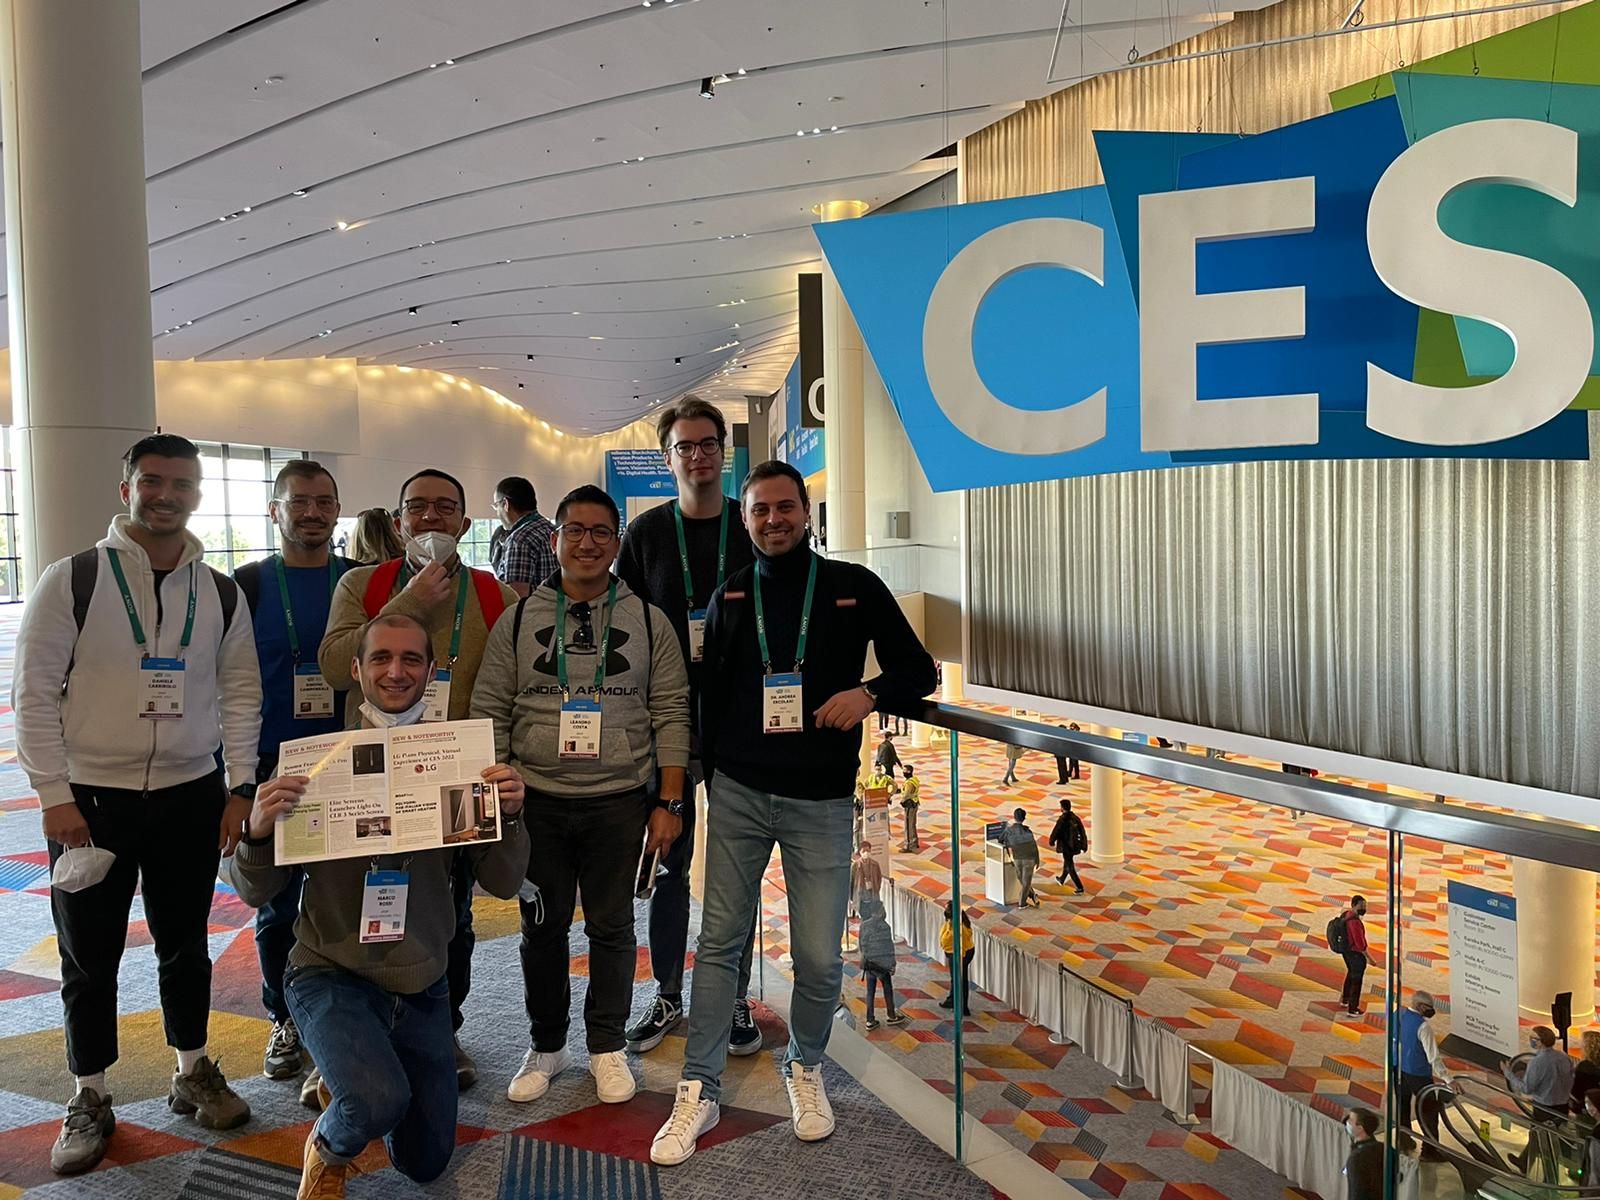
\includegraphics[width=12cm]{img/ces.jpeg}
    \caption{IRSAP ed IOTINGA al CES 2022}
    \label{fig:ces}
\end{figure}

\section{Necessità di test di un dispositivo IoT}

La caratteristica fondamentale per questi prodotti è l'affidabilità.
Infatti nessun utente installerebbe in casa propria un dispositivo che
non è in grado di svolgere la funzione per la quale è stato acquistato.

A maggior ragione i danni derivanti dal malfunzionamento di un impianto
di riscaldamento possono coinvolgere non solo cose ma anche estendersi
a persone ed animali domestici.

È tassativo prestare attenzione alle problematiche che si possono verificare
in utenza, le quali non sono solo un danno per il cliente stesso ma anche
per l'azienda produttrice:

\begin{itemize}
\item la prima impressione sul cliente è quella che conta, se il cliente si ritrova
    un prodotto che funziona male o addira non svolge la funzione prevista ne parlerà
    male, anche mediante recensioni negative online, e creerà un danno d'immagine all'azienda
    difficilissimo da sanare
\item quando il problema si verifica dal cliente è complicata la diagnostica. I clienti,
    e spesso anche gli installatori stessi, non hanno competenze tecniche o il
    tempo da dedicare nel supportare il produttore nella ricerca del problema
\item se il problema non è risolvibile mediante un aggiornamento firmware è necessario
    effettuare un reso, che ha dei costi molto elevati per il produttore, in quanto
    durante il trasporto molto spesso il prodotto viene danneggiato e quindi deve
    essere rimpiazzato con un nuovo
\end{itemize}

È di fondamentale importanza assicurarsi di identificare il prima possibile quanti
più problemi possibili prima che il prodotto arrivi nelle mani dell'utente finale.

In tutto questo il software ricopre un ruolo sempre più da protagonista, in quanto
per garantire la connettività al cloud è necessario gestire una complessità elevata.

I prodotti della precedente generazione utilizzavano il software per una mera gestione
delle periferiche fisiche del prodotto, senza la necessità di interfacciarsi con sistemi
terzi. Al contrario i prodotti della attuale per svolgere tutte le funzioni di
integrazione cloud in maniera sicura richiedono un livello aggiuntivo di astrazione,
ovvero quello di un RTOS (sistema operativo real-time).

Anche l'hardware stesso è più evoluto, infatti si passa dalle piattorme ad 8 bit ai
microcontrollori a 32, con funzionalità sempre più assimilabili a quelle di un sistema
general purpose, quali ad esempio una gestione di programmazione concorrente, uno
stack di rete TCP/IP, ed una gestione della memoria virtual con MMU.

Un'altra differenza rispetto al passato è la possibilità di aggiornare il software dopo
che il prodotto lascia la fabbrica, mediante aggiornamenti di tipo ``Over The Air'' (OTA).
Questo si rende necessario non solo per la mera introuduzione di nuove funzionalità in
un prodotto esistente, ma anche per mantenere il software al passo con l'evoluzione degli
altri sistemi a cui esso si collega, quale ad esempio modifiche nei protocolli di rete
dettate dall'arrivo di nuovi standard.

Sebbene l'aggiornamento consenta di risolvere problemi dopo che il dispositivo ha lasciato la
fabbrica esso comporta anche una criticità, in quanto vi è il rischio di introdurre altri problemi
in prodotti che fino a quel momento non li avevano, andando a creare un disservizio.

Bisogna infine tener conto che un prodotto di questo tipo segue un ciclo di vita molto lungo
rispetto ad esempio a PC o smartphone, che può tranquillmente superare i 10 anni dalla data di
immissione nel mercato, e l'utente si aspetta che in tutti questi anni possa continuare ad
utilizzarlo come il giorno in cui lo ha acquistato.

Conseguentemente diventa prioritario garantire i massimi livelli di qualità possibile
sul software rilasciato. Questo non si limita alla semplice assenza di bug, in quanto
questa è una garanzia che matematicamente è impossibile offrire, ma anche all'adottare
delle procedure procedure tali che consentano, dal momento che un bug si
presenta, di individuarlo e sistemarlo nel minor tempo possibile.

Tracciabilità e mantenibilità del codice sono quindi parole chiave, la prima garantisce che
sia sempre possibile risalire all'esatta versione del codice per il quale viene segnalato un
problema di modo da poterlo riprodurre, la seconda invece assicura che la soluzione al problema
sia implementabile nel minor tempo possibile e senza il rischio di regressioni.

Infine l'altro punto cardine è l'eseguire test metodologici prima che il firmware venga
rilasciato al pubblico, sia tramite aggiornamento OTA che tramite installazione in fabbrica
su di un nuovo prodotto.

\subsection{Prassi attuale testing}

Allo stato attuale abbiamo 3 momenti di validazione di un rilascio:

\begin{enumerate}
    \item test da parte dello sviluppatore
    \item test di accettazione interna (in IOTINGA)
    \item test di accettazione del cliente finale (IRSAP)
\end{enumerate}

\subsection{Test di sviluppatore}

Quando uno sviluppatore finisce di implementare una nuova funzionalità o risolve un
bug  prima di considerare l'attività conclusa ed integrare il
proprio lavoro nel ramo di sviluppo principale ed effettua i propri test.

Questi si occupano sia di verificare che quanto è stato implementato è conforme
alla specifica approvata dal cliente (nel caso di nuove funzionalità) oppure che
il bug sia stato risolto, sia che non siano stato modificato il funzionamento del sistema
nelle parti che sono state impattate dalla modifica.

Tali test sono a discrezione dello sviluppatore, che avendo modificato il codice sa
quali comportamenti sono impattati dalla modifica che ha realizzato e quindi devono essere
provati.

Questi test possono essere automatizzati facilmente mediante la creazione di unit-test, 
che possono essere usati per validare sia le parti nuove che assicurarsi che non vi siano 
regressioni che fanno smettere di funzionare quanto prima andava. 

\subsection{Test di accettazione interna}

Questi test sono effettuati prima di ogni rilascio verso il cliente IRSAP.

Si occupano di validare che il software garantisca il funzionamento di una serie di casi d'uso
definiti critici, senza i quali il prodotto non sarebbe utilizzabile.
Solo se una versione del software passa tutti questi test può essere consegnata al cliente.

Essi si pongono dal punto di vista dell'utente finale, pertanto sono effettuati su un
hardware completo, isolato però dal resto del sistema, ovvero dalla componente cloud
e dall'applicazione mobile. Questo per evitare che ci sia il dubbio che il bug sia
nel cloud o nella app anziché nel dispositivo stesso.

Attualmente vengono effettuati seguendo un documento contenente una serie di scenari da testare. 
Ognuno di questi è diviso in passi, e per ognuno dei quali viene indicato:

\begin{itemize}
    \item azione da compiere: un'operazione da effettuare sul sistema mediante l'interazione fisica
        con il dispositivo (pressione di pulsanti) oppure mediante cloud (tramite un apposito
        strumento che consente di simulare i messaggi inviati dal cloud e dalla app)
    \item risultato atteso: postcondizioni da verificare dopo aver effettuato l'azione, espresso in 
        linguaggio non formale, ad esempio ``i led sono rossi'' oppure ``entro 5 secondi viene inviato al cloud un messaggio''.
        Nel caso la postcondizione sia verificata è possibile procedere al passo successivo, altrimenti
        il test viene interrotto con esito negativo, e deve essere segnalato ad uno sviluppatore il problema.
\end{itemize}

Preferibilmetne questa procedura viene fatta eseguire da chi non ha preso parte allo
sviluppo del sistema stesso. Questo per evitare che chi esegue la procedura, conoscendo
le logiche interne del software, possa essere portato a saltare o ignorare determinati
passaggi in quanto ``ovvi'', mentre chi non conosce il sistema è più propenso a seguire
i passaggi alla lettera e segnalare ogni singolo comportamento discordante con quanto
atteso.

\subsection{Test di accettazione del cliente finale}

Sul cliente finale ricade la responsabilità (anche a livello legale) del prodotto
che viene immesso sul mercato con il proprio nome sopra, e questo include anche
il software. Questo comporta il fatto che a sua volta deve svolgere dei test per
assicurarsi che il software sia conforme a quanto atteso, e nel caso segnalare i
problemi riscontrati in maniera tale che vengano corretti.

Questi test sono volti a testare tutte le funzionalità del prodotto in tutte le loro
possibili configurazioni, anche mediante l'ausilio di strumentazione altamente
specializzata quali camere climatiche per valutarne l'efficacia di termoregolazione.

Nel caso questi test abbiano successo l'artefatto testato passa da stato di candidato
al rilacio a produzione, e viene quindi installato in fabbrica su tutti i nuovi radiatori
prodotti, nonché viene lanciato un aggiornamento OTA su tutti i dispositivi già installati
presso i clienti finali.

\section{Problemi aperti dell'approccio attuale di test di accettazione}

L'approccio attuale, basato sul documento di test con fasi da seguire, presenta
alcune problematiche:
\begin{itemize}
    \item la procedura è ripetitiva, e questo può facilmente introdurre
        l'operatore che esegue i test a commettere errori, con dolo o meno
    \item l'esecuzione dei test porta via tempo, che altrimenti potrebbe essere dedicato 
        a svolgere altre mansioni
    \item i test sono scritti in linguaggio naturale, non formale, e questo lascia spazio 
        a libera interpretazione dalla persona che esegue i test
    \item il fatto che sia un costo eseguire la procedura fa sì che questa sia
        limitata nel numero di scenari che sono effettivamente testati
    \item per quanto detto al punto precedente il numero di build effettivamente testate 
        è un sottoinsieme di quelle che vengono effettivamente effettuate, il che significa che 
        i rilasci verso il cliente avvengono con meno frequenza, e si tende ad accorpare 
        più funzionalità in maniera tale da effettuare un unico ciclo di test. 
\end{itemize}

A questo si aggiunge il fatto che man mano che i prodotti vengono venduti il cliente ci 
chiede sempre più test ad ogni release, in quanto un potenziale bug va ad impattare un numero 
sempre maggiore di utenti (e quindi il danno potenziale per il produttore è sempre più grande). 

Viene quindi da chiedersi se, vista la ripetitività e schematicità di queste operazioni,
sia possibile farle eseguire ad un computer, senza perdite di generalità rispetto all'esecuzione 
manuale.

\section{Requisiti di un sistema di esecuzione di test di accettazione automatici}

Abbiamo quindi stabilito i seguenti requisiti per un sistema di automatizzazione dei test di 
accettazione:

\begin{itemize}
    \item il sistema deve testare esattamente il binario che poi viene rilasciato agli utenti finali. 
        Questo perché ogni alterazione, come potrebbe essere una ricompilazione del codice, può andare 
        ad aggiungere errori e quindi invalidare i test effettuati
    \item l'ambiente di esecuzione (runtime environment) sul quale il test viene eseguito deve essere quanto 
        più vicino possibile all'ambiente reale. Idealmente il test viene effettuato sullo stesso hardware, 
        di modo da divanare ogni possibile dubbio che il firmware una volta installato sull'hardware abbia 
        comportamenti differenti
    \item l'ambiente deve poter eseguire il firmware in differenti configurazioni di hardware che esso supporta
        (attualmente supporta due tipologie di hardware, e ne verranno aggiunte altrettante due a breve)
    \item il sistema deve avere abbastanza flessibilità per poter validare almeno le funzionalità che oggi 
        sono teste manualmente
    \item deve essere sufficientemente semplice andare ad aggiungere nuovi scenari e configurazioni da provare al sistema
    \item deve essere possibile integrare lo strumento all'interno del flusso di CI/CD attualmente in 
        uso in azienda, di modo che ogni release del firmware prodotta venga testata senza necessità di 
        un intervento manuale
\end{itemize}

\chapter{Lavori correlati}

Vediamo ora cosa è disponibile in commercio per fare quanto descrito al capitolo precedente. 

\section{Strumenti di unit test}

Una prima soluzione è quella di utilizzare gli strumenti di 
unit-test anche per effettuare i test di accettazione. 
È possibile infatti andare ad effettuare il mock di tutte le interfacce utilizzate dall'SDK
al fine di poter eseguire singoli test-case all'interno del binario. 

Questa soluzione presenta il vantaggio di poter testare in maniera veloce ed agevole 
ogni nuova release del firmware, ma al contempo presenta alcuni svantaggi che la rendono
inadatta allo scopo di approvare un nuovo firmware per la produzione. 

Il problema principale è che viene testato il codice facendolo girare in un ambiente simulato,
che per quanto simile all'ambiente reale non sarà mai completamente uguale. Soprattutto 
quando ci si interfaccia con periferiche complesse, come il Wi-Fi, è fondamentale che 
l'ambiente sul quale vengono eseguiti i test sia quanto più uguale possibile al runtime effettivo. 

In questo caso la soluzione migliore è effettuare i test facendo eseguire il firmware direttamente 
all'hardware sul quale dovrà girare. 

\section{Strumenti commerciali di test elettronici}

In commercio esistono vari strumenti che consentono di testare un dispositivo elettronico andando 
a comandare i vari input/output con i quali si interfaccia verso il mondo esterno. 

Uno di questi software è TestStand della National Instrument\footnote{https://www.ni.com/it-it/shop/software/products/teststand.html}. 
Questo software è infatti pensato per l'interfacciamento con apparecchiature di misura prodotte 
dalla medesima azienda, quali ad esempio oscilloscopi, multimetri da banco, generatori di frequenza, ecc. 
e consente di automatizzare le operazioni di test e misura. 

Come questo esistono altri software, principalmente proprietari e sviluppati internamente dalle singole 
aziende elettroniche, che svolgono la medesima funziona. Questi software tipicamente si interfacciano 
con la scheda hardware attraverso una fixture, composta da un letto di aghi conduttivi che vanno a 
fare contatto con dei test-point sulla scheda da testare. 

Questi sistemi possono benissimo essere utilizzati anche per testare il firwmare. Tuttavia non è 
il loro scopo primario, essendo pensati per identificare in primo luogo diffetti nella produzione 
fisica delle schede. In particolare non offrono routine per testare componenti complesse come Wi-Fi o comunicazione con il 
cloud, ma si limitano a fare verifiche fra gli input e gli output. 

Inoltre l'hardware di questi dispositivi è molto costoso, essendo pensato per effettuare misurazioni 
precise a livello fisico, cosa che è fondamentale per identificare diffetti sull'hardware, ma lo è 
meno per testare la release del firwmare (dove si assume che l'hardware sul quale viene lanciato il test 
sia correttamente funzionante). 

\section{Conclusioni}

In generale abbiamo visto che il software che rispondeva ai nsotri requisiti non esisteva già sul mercato, 
sia come software commerciale che come software open-source. 

\chapter{Approccio}

Prima di descrivere l'implementazione è necessario fare un passo indietro ed andare 
ad analizzare con più attenzione il dispositivo radiatore elettrico preso in esame. 

\section{Caratteristiche hardware}

Tutta la linea di radiatori elettrici smart IRSAP (che attualmente si compone di 17 prodotti distinti,
in continua espansione) utilizza al suo interno la stessa elettronica, che attualmente viene 
prodotta in due varianti:

\begin{itemize}
    \item \textit{luxury}: è la versione più basilare, che viene utilizzata sulla linea di 
        radiatori da bagno (gli scaldasalviette). 
    \item \textit{design}: è la versione riservata ai prodotti design. È la versione più completa, 
        ed offre, in aggiunta a tutto quanto offerto dalla \textit{luxury}, un sensore di qualità
        dell'aria (in grado di rilevare i valori di VOC e CO\textsubscript{2}) e la possibilità di
        controllare una striscia LED RGBW, utilizzata in alcuni radiatori per questioni
        di illuminazione estatica.
\end{itemize}

Inoltre a parità di elettronica un radiatore può o meno avere a disposizione le
seguenti funzionalità:
\begin{itemize}
    \item Fil Pilote: uno standard francese per l'interconnessione dei radiatori ad una
        centralina di controllo mediante un secondo ingresso di segnale a 230V
    \item LED RGBW: disponibili solo su radiatore con scheda design, consente di
        illuminare l'ambiente circostante al radiatore per creare atmosfera
\end{itemize}

Sulla scheda trovano spazio i seguenti componenti:

\begin{itemize}
    \item un modulo Wi-Fi Telit GS2200M
    \item circuito di alimentazione a 230V AC
    \item un circuito composto da un relè più un triac dedicato al controllo della
        cartuccia, ossia l'elemento riscaldante inserito all'interno del corpo del radiatore
    \item una sonda di temperatura NTC usata per rilevare la temperatura ambiente
    \item una pulsantiera dotata di due pulsanti capacitivi e dei led RGB di illuminazione
        come feedback verso l'utente
    \item un buzzer utilizzato per dare un feedback uditivo all'utente
    \item solo per le schede \textit{design} un sensore di qualità dell'aria in grado di
        misurare i livelli VOC e CO\textsubscript{2}
    \item un ingresso per il segnale ``Fil Pilote'' (solo per i modelli che lo prevedono)
    \item la circuiteria di controllo per una striscia a led RGBW di illuminazione ambientale
    \item la circuiteria di controllo per una seconda sonda di temperatura in grado di
        misurare la temperatura del corpo riscaldante, in maniera tale da migliorare
        l'accuratezza degli algoritmi di termoregolazione
\end{itemize}

Tutte le versioni di scheda elettronica eseguono la stessa versione del firmware,
che ha una fase iniziale in cui identifica la tipologia di scheda e le funzionalità
opzionali abilitate leggendole da un file di configurazione caricato nel dispositivo
in fase di collaudo, e di conseguenza configura le periferiche del microcontrollore.

Tuttavia per essere esaustivi è necessario svolgere i test di accettazione su entrambe
le versioni di scheda elettronica, in quanto possono esservi comportamenti differenti.

\subsection{Modulo Telit}

Come cuore del sistema abbiamo il GS2200M. Questo microcontrollore inizialmente
prototto da Gainspan, successivamente acquisita da Telit, presenta le seguenti
caratteristiche hardware:

\begin{itemize}
    \item processore dual core ARM Cortex M3 fino a 120Mhz, di cui un core dedicato
        alla gestione del Wi-Fi ed uno all'esecuzione dell'applicativo
    \item 1Mb di RAM in totale, di cui all'incirca 500kB utilizzabile dall’applicazione,
        il resto dedicata all'uso della parte Wi-Fi
    \item 4Mb di memoria flash interna, in parte dedicata al codice del firmware ed
        in parte come filesystem interno in cui memorizzare i dati dell'applicazione
    \item interfaccia Wi-Fi b/g/n a 2.4Ghz in grado di operare sia in modalità station
        (client) sia che access-point (AP) a cui connettersi direttamente
    \item 19 input/output digitali
    \item 3 output PWM
    \item 2 ingressi analogici mediante ADC, uno a 10 ed uno a 12 bit
    \item un interfaccia I2C hardware
    \item un interfaccia SPI hardware
    \item due interfacce seriali UART
    \item modulo RTC interno
\end{itemize}

Il microcontrollore è dostato due due core ARM, di cui uno è deputato alla gestione
della parte Wi-Fi ed esegue un firmware scritto dal produttore stesso. I due microcontrollori
comunicano attraverso una memroia condivisa (dual-port) da 64Mb. Il core principale
si occupa invece di gestire la parte applicativa.

La toolchain fornita dal produttore per lo sviluppo del firmware in grado di girare
sul core applicativo si basa sull'ambiente di sviluppo proprietario IAR.

Viene fornito un SDK che offre:

\begin{itemize}
    \item un sistema operativo real-time (\textit{RTOS}) basato su ThreadX
    \item uno stack di rete TCP/IP basato su NetX
    \item implementazione software Wi-Fi sia in modalità station (STA) che access-point (AP),
        con relativi protocolli WEP, WPA/WPA2 sia personal che enterprise
    \item un filesystem (simile al FAT32) per la gestione della memoria flash integrata
    \item implementazione TLS
    \item implementazione client e server del protocollo HTTP ed HTTPS
    \item implementazione client del protocollo SNTP
    \item aggiornamento OTA con doppia partizione
    \item hardware abstraction layer (HAL) per la gestione di tutti i GPIO,
        lettura dei due ADC, del modulo PWM, gestione del RTC, del bus i2c ed SPI
\end{itemize}

I moduli Wi-Fi di questo tipo possono essere utilizzati secondo due modalità:
\begin{itemize}
    \item \textit{hosted}: il modulo Wi-Fi viene interfacciato ad un microcontrollore
        principale che implementa le funzioni del dispositivo. Quest'ultimo si interfaccia
        con il Telit mediante interfaccia seriale e comunica con i comandi AT (standard
        per la gestione dei modem)
    \item \textit{hostless}: il modulo Wi-Fi esegue direttamente l'applicativo senza
        che vi sia un microcontrollore principale. Tutte le funzionalità del dispositivo
        sono impelementate sul modulo Telit
\end{itemize}

Tipicamente viene seguito il primo approccio, tuttavia noi abbiamo optato per il secondo.
Questo comporta svariate semplificazioni, quali il non dover gestire la distribuzione
e l'aggiornamento di due firmware, e l'avere quindi un prodotto più solido.

Un secondo microcontrollore comporta inoltre problemi di approvvigionamento, soprattutto di
questi ultimi periodi in cui il mercato dei componenti elettronici è impazzito, con
articoli che un tempo costavano pochi dollari arrivati a costare svariate decine.

La scelta di seguire l'approccio \textit{hostless} non è stata senza difficoltà, dovute
principalmente alla scarsa documentazione fornita dal produttore Telit. Infatti il
produttore ha deciso di seguire un approccio completamente closed-source, dove tutta
la documentazione ed il codice di esempio non è pubblico ma dato solo sotto NDA.

Questo comporta che l'unico modo per risolvere i problemi sia quello di rivolgersi
al supporto ufficiale, non trovando nulla riguardo questa particolare piattaforma
hardware con una semplice ricerca su Google. Questo ha indubbiamente reso molto più
difficoltoso lo sviluppo.

\section{Caratteristiche software}

Il firmware è suddiviso in moduli (task):

\begin{itemize}
    \item \textit{core}, si occupa della gestione della macchina a stati principale
        del dispositivo e del coordinamento di tutti gli altri task. Inizializza tutte
        le periferiche hardware e la rete, oltre che gestire
        gli eventi notevoli che arrivano dagli altri task
    \item \textit{termostato}, task che si occupa di tutto quel che è necessario
        per regolare la temperatura ambiente secondo le modalità di funzionamento del dispositivo,
        della lettura delle sonde ambiente/VOC, non che della gestione dell'illuminazione LED
        nel caso sia presente
    \item \textit{AWS}, si occupa di mantenere la connessione MQTT verso AWS IoT Core,
        sincronizzato lo stato interno del dispositivo con il server ``IRSAP NOW'' mediante protocollo MQTT
    \item \textit{hmi}, si occupa di rispondere agli input dell'utente
        sulla pulsantiera e di darne relativo feedback mediante l'uso dei LED RGB e del buzzer
    \item \textit{HTTP}, si occupa di fornire mediante webserver HTTP un'API REST con
        la quale è possibile interagire direttamente con il dispositivo. È utilizzata
        per la fase di provisioning.
    \item \textit{NCM}, si occupa di gestire la connessione di rete Wi-Fi. Questo task
        è fornito dal produttore.
\end{itemize}

\subsection{Stati interni del dispositivo}

Il dispositivo ad alto livello può trovarsi in 3 stati distinti:

\begin{itemize}
    \item \textit{non abbinato}: in attesa di un primo abbinamento da app. Ogni funzione del
        dispositivo è esclusa finché l'utente non lo collega mediante l'applicazione
    \item \textit{disconnesso}: il dispositivo è stato in passato abbinato ma al momento non è
        connesso al cloud, perché ad esempio la connessione Wi-Fi non è momentaneamente disponibile
    \item \textit{connesso}: il dispositivo è connesso e sincronizzato con il cloud
\end{itemize}

\begin{figure}[ht]
    \centering
    \begin{tikzpicture}
        \node[state] (unbounded) {Non abbinato};
        \node[state, below left of=unbounded, below=1cm] (offline) {Disconnesso};
        \node[state, right of=offline] (online) {Connesso};
        \draw (unbounded) edge[bend left, align=left, right] node{abbinato\\con successo} (online)
        (offline) edge[bend left, above] node{connessione} (online)
        (offline) edge[bend left, left, align=right] node{ripristino\\di fabbrica} (unbounded)
        (online) edge[bend left, below] node{disconnessione} (offline)
        (online) edge[bend left, align=right, right] node{ripristino\\di fabbrica} (unbounded);
    \end{tikzpicture}
    \caption{Stati del radiatore}
    \label{fig:stati}
\end{figure}

Ad ogni stato del dispositivo corrisponde l'attivazione/disattivazione di uno o più
componenti software del dispositivo:

\begin{center}
\begin{tabular}{| c | c | l |}
    \hline
    stato & modo Wi-Fi & moduli attivi \\
    \hline
    \textit{non abbinato} & AP & HMI, HTTP \\
    \hline
    \textit{disconnesso} & client & HMI, termostato \\
    \hline
    \textit{connesso} & client & HMI, termostato, AWS \\
    \hline
\end{tabular}
\end{center}

\subsection{Termoregolazione}

La componente di termoregolazione si occupa di regolare la temperatura ambiente portandola
il più vicino possibile a quanto desiderato dall'utente (set-point) mediante
il controllo dell'accensione (on/off) dell'elemento riscaldante. Il feedback sulla
temperatura ambiente è ottenuto mediante la sonda di temperatura NTC.

Il dispositivo ha diversi modi di funzionamento:
\begin{itemize}
    \item standby: dispositivo completamente spento, sia per quanto riguarda il riscaldamento
        che per l'illuminazione LED
    \item antigelo: il dispositivo mantiene una temperatura di sicurezza (impostata dall'utente)
        per prevenire danni dati da una tempratura ambiente troppo bassa (ad es. congelamento delle tubature)
    \item vacanza: all'interno di un intervallo temporale impotato dall'utente funziona
        in modalità antigelo
    \item away: imposta un set-point ridotto (ECO) in quanto l'utente non è in casa
    \item programmato: segue una programmazione settimanale che consente per ogni
        giorno della settimana di creare fino ad 8 fasce orarie
    \item manuale temporaneo: segue un set-point manuale per un determinato tempo
    \item manuale: segue il set-point utente che è fisso e non varia mai
        configurato dall'utente, quindi torna a funzionare nella modalità precedente
    \item fil pilote: il dispositivo è controllato (ove disponibile) da un segnale
        esterno in ingresso sul cavo fil pilote
\end{itemize}

È possibile mediante interfaccia utente muoversi fra le varie modalità come dettagliato
in \autoref{fig:modi}.

\begin{figure}[ht]
    \centering
    \begin{tikzpicture}
        \node[state] (programmato) {Programmato};
        \node[state, right of=programmato, align=center] (manuale-tempo) {Manuale\\temporaneo};
        \node[state, right of=manuale-tempo] (manuale) {Manuale};
        \draw (manuale) edge[loop above] node{modifica set-point} (manuale)
            (programmato) edge[bend left, above] node{modifica set-point} (manuale-tempo)
            (manuale-tempo) edge[bend left, above] node{modifica set-point} (manuale);
    \end{tikzpicture}
    \caption{Modi del radiatore}
    \label{fig:modi}
\end{figure}

\subsection{Comunicazione cloud}

La componente cloud è implementata su AWS. La connessione avviene grazie al protocollo
MQTT usando il servizio broker di AWS, IoT Core.

\subsubsection{Autenticazione}
La connessione è cifrata mediante TLS 1.2 ed autenticata mediante certificato del client. 

Tale certificato è generato per ogni singolo dispositivo durante le fasi di produzione, 
e viene firmato da una CA intermedia del produttore hardware, come nel seguente schema: 

\begin{figure}[ht]
    \centering
    \begin{tikzpicture}
        \node[rectangle, draw, align=center, inner sep=8pt] (root) {root CA \\AWS};
        \node[rectangle, draw, right of=root, align=center, inner sep=8pt] (intermedia) {CA intermedia\\ produttore};
        \node[rectangle, draw, right of=intermedia, align=center, inner sep=8pt] (dispositivo) {certificato TLS\\ dispositivo};
        \draw (root) edge[above] node{firma} (intermedia)
            (intermedia) edge[above] node{firma} (dispositivo);
    \end{tikzpicture}
    \caption{Catena TLS}
    \label{fig:tls-chain}
\end{figure}

La CA autority intermedia è generata e firmata dalla CA generale di AWS IoT Core. In questo 
modo è possibile generare in fase di programmazione offline un certificato per ogni 
dispositivo che deve essere prodotto. Alla prima connessione del dispositivo al cloud questo 
automaticamente si registrerà all'interno di IoT Core senza ulteriori necessità di interventi manuali. 

IoT Core permette di associare ad ogni certificato una policy, che può andare a garantire al 
client dei permissi per quanto riguarda MQTT:
\begin{itemize}
    \item \textit{connect}: autorizza il client a connettersi ad IoT Core utilizzando un particolare 
        \textit{clientId}
    \item \textit{publish}: consente al cilent di pubblicare su determinati topic MQTT
    \item \textit{subscribe}: consente al dispositivo di effettuare una subscription su determinati topic 
        al fine di ricevere aggiornamenti in tempo reale dal cloud
\end{itemize}

La policy predefinita restringe i permessi ai soli topic dedicati per il client con il determinato certificato 
che si connette al cloud. Per fare questo all'interno del topic viene inserito il seriale dello specifico 
dispositivo, che è lo stesso contenuto all'interno del certificato. 

\subsubsection{Protocollo stateless di comunicazione}

Per quanto concerne il protocollo di comunicazione in origine abbiamo valutato inizialmente 
l'uso del protocollo Device Shadowing\footnote{\url{https://docs.aws.amazon.com/it\_it/iot/latest/developerguide/iot-device-shadows.html}} 
supportato nativamente da AWS IoT Core. 

Tuttavia, tale protocollo aveva delle limitazioni che non ne consentivano l'utilizzo nella nostra
applicazione, in particolare:

\begin{itemize}
    \item il pacchetto viene codificato in JSON, il che presenta un overhead di memoria
        e CPU notevole per il microcontrollore scelto. Inoltre la codifica JSON può
        introdurre dei bug di encoding
    \item vi è un hard-limit di 8Kb di dimensione massima di un documento di stato (shadow).
        Questo, seppur poteva essere sufficiente nelle prime versioni del prodotto, andava
        a limitare possibilità di espansione futura del prodotto
    \item il protocollo di comunicazione trasferisce dei delta, che sebbene riducano la
        dimensione di un pacchetto di dati rendono più complessa la sincronizzazione degli
        stati del sistema
\end{itemize}

Per tutte queste ragioni abbiamo scelto di adottare un protocollo binario proprietario,
tramite il quale andiamo a trasferire stati completi del dispositivo.

Abbiamo deciso di mantenere comunque i concetti di alto livello dati dal protocollo AWS
Device Shadowing, in particolare la nomenclatura \textit{shadow} per indicare uno stato del 
dispositivo, che è suddiviso in:
\begin{itemize}
    \item \textit{state desired} come lo stato in cui si vuole portare il dispositivo, ovvero le
        impostazioni che l'utente può modificare agendo dalla app, quali ad esempio la modalità di funzionamento,
        la programmazione oraria, la configurazione dei LED RGB, etc.
    \item \textit{state reported} lo stato attuale del dispositivo. È un superset dello stato
        desired, in quanto oltre a tutti i campi di quest'ultimo include anche tutti quei valori
        in sola lettura (ovvero che solo il dispositivo può modificare), ovvero i parametri
        statistici e di monitoraggio quali la temperatura ambiente, il livello di qualità dell'aria (VOC),
        gli allarmi del dispositivo, la qualità della connessione Wi-Fi, etc.
\end{itemize}

Il protocollo è quindi stateless, e consente di effettuare 4 messaggi, più relative risposte,
(come visibile in \autoref{fig:comunicazione_cloud}):

\begin{itemize}
    \item \textit{get}: disponibile fra dispositivo e cloud, consente la richiesta dello stato \textit{desired} corrente
    \item \textit{reported-update}: disponibile fra dispositivo e cloud, trasmette lo stato
        completo del dispositivo al server
    \item \textit{delete}: eliminazione dello stato corrente presente su cloud
    \item \textit{desired-udpate}: unico messaggio inviato dal cloud al dispositivo,
        trasmette lo stato completo desired
\end{itemize}

Il tipo di messaggio dipende dal topic MQTT sul quale i pacchetti sono pubblicati. Ad
un messaggio pubblicato dal dispositivo verso il server il server risponde in base allo
stato della richiesta sullo stesso topic con aggiunto un suffisso:
\begin{itemize}
    \item \texttt{/accepted}: la richiesta è stata accettata dal server
    \item \texttt{/rejected}: la richiesta è stata respinta dal server in quanto è 
        avvenuto un errore
\end{itemize}

\begin{figure}[ht]
    \centering
    \begin{tikzpicture}
        \node[rectangle, minimum height=1cm, draw] (dispositivo) {Radiatore Elettrico};
        \node[rectangle, minimum height=1cm, draw, right of=dispositivo] (cloud) {Cloud AWS};
        \draw (dispositivo) edge[bend left=40, above] node{\textit{get}} (cloud)
            (dispositivo) edge[bend left=10, above] node{\textit{reported-update}} (cloud)
            (dispositivo) edge[bend right=10, below] node{\textit{delete}} (cloud)
            (cloud) edge[bend left=40, below] node{\textit{desired-update}} (dispositivo);
    \end{tikzpicture}
    \caption{Schema di comunicazione dispositivo/cloud}
    \label{fig:comunicazione_cloud}
\end{figure}

Il client può identificare a quale richiesta fa riferimento ad una risposta attraverso un
token (\textit{clientToken}) che il client setta su ogni richiesta inviata e che il server aggiunge
ad ogni risposta che invia al client.

\subsubsection{Formato messaggi cloud}

Ogni messaggio su cloud include un header fisso, che comprende i seguenti campi

\begin{center}
\begin{longtable}{| p{5cm} | c | p{8cm} |}
    \hline
    \textbf{campo} & \textbf{tipo} & \textbf{descrizione} \\ \hline
    timestamp & u32 & timestamp di invio del messaggio \\ \hline
    clientToken & u32 & un ID della richiesta che il client aggiunge ad ogni messaggio
        per poter correlare le risposte alle richieste effettuate \\ \hline
    version & u32 & versione del messaggio \\\hline
    length & u16 & lunghezza totale del messaggio (header incluso) \\ \hline
    type & u8 & tipo di messaggio, identifica il payload presente \\ \hline
\end{longtable}
\end{center}

A seguire nel messaggio è presente il payload:

\begin{center}
\begin{longtable}{| p{5cm} | c | p{8cm} |}
    \hline
    \textbf{campo} & \textbf{tipo} & \textbf{descrizione} \\ \hline
    connected & u8 & 1 se il dispositivo è online, altrimenti 0 \\ \hline
    firmwareVersion & u8[2] & versione firmware (major, minor) \\ \hline
    hardwareVersion & u8 & versione hardware \\ \hline
    macAddress & u8[6] & MAC address (ID dispositivo) \\ \hline
    systemStatus & u8 & stato del Sistema (bitmask) \\ \hline
    filPiloteStatus & u8 & stato ingress Fil Pilote \\ \hline
    alarm & u8 & allarmi (bitmask)\\ \hline
    heatingStatus & u8 & stato riscaldamento (bitmask)\\ \hline
    rssi & u8 &Potenza Wi-Fi\\ \hline
    noise & u8 &Rumore Wi-Fi\\ \hline
    currentSetPoint & i16 & set point corrente (in decimi di grado)\\ \hline
    currentSetPointEnd & u32 & scadenza set-point corrente\\ \hline
    vocValue & u16 & valore VOC (qualità dell’aria)\\ \hline
    co2Value & u16 & valore CO2 (qualità dell’aria)\\ \hline
    temperature & i16 & temperature ambiente (in decimi di grado)\\ \hline
    setPointOff & u16 & set point di OFF (in decimi di grado)\\ \hline
    setPointEco & u8 & set point di ECO (in decimi di grado)\\ \hline
    manualSetPoint & u8 & set point manual (in decimi di grado)\\ \hline
    temporaryManualSetPoint & u8 & set point manual temporaneo (in decimi di grado)\\ \hline
    temporaryManualEnd & u32 & fine manuale temporaneo (timestamp)\\ \hline
    hysteresis & u8 & isteresi (+/- decimi di grado)\\ \hline
    temperatureSensorOffset & i8 & correzione sensore di temperature (in decimi di grado)\\ \hline
    loadTemperature & i16 & temperature carico (in decimi di grado)\\ \hline
    loadOnSeconds & u32 & cumulativo in secondi di accensione del carico\\ \hline
    holidayStart & u32 & timestamp inizio vacanza\\ \hline
    holidayEnd & u32 & timestamp fine vacanza\\ \hline
    metricInterval & u8 & intervallo invio metriche periodiche (minuti)\\ \hline
    systemId & u8[16] & ID impianto (UUID)\\ \hline
    timezone & i16 & offset timezone rispetto ad orario UTC\\ \hline
    systemConfiguration & u8 & configurazione di sistema (bitmask)\\ \hline
    ipAddress & u8[4] & indirizzo IP Wi-Fi\\ \hline
    openWindowOffTime & u8 & tempo di spegnimento in caso rilevamento finestra aperta\\ \hline
    ledManualSetPoint & u32 & colore LED ambiente (HSV)\\ \hline
    schedule & u8[196] & programmazione riscaldamento\\ \hline
    ledSchedule & u8[196] & programmazione LED (stesso formato di prima)\\ \hline
    ledEnabled & u8 & LED ambiente on/off\\ \hline
    ledMode & u8 & modalità led ambiente (manuale/programmato)\\ \hline
    ledColor & u32[10] & preset colori LED ambiente per uso in fasce orarie\\ \hline
    temporaryManLedSP & u32 & set point LED manuale a tempo\\ \hline
    temporaryManLedSPEnd & u32 & fine manuale a tempo LED\\ \hline
    estimatedTemperature & i16 &temperatura ambiente (scritta da cloud per uso con altri sensori)\\ \hline
    externalTemperature & i16 & umidità esterna (scritta da cloud)\\ \hline
    estimatedHumidity & u8 & umidità ambiente (scritta da cloud)\\ \hline
    externalHumidity & u8 & umidità esterna (scritta da cloud)\\ \hline
    currentLedSetPoint & u32 & set point LED corrente\\ \hline
    currentLedSetPointEnd & u32 & fine fascia oraria LED corrente\\ \hline
    cartridgePowerWatts & u16 & potenza della cartuccia\\ \hline
    cumuConsumption & u32 & consumo cumulato in tutta la vita del radiatore\\ \hline
    cumuConsumptionValue & u32 & valore all’ultimo snapshot di constumo\\ \hline
    cumuConsumptionTime & u32 & consumo all’ultimo snapshot\\ \hline
    modelName & char[32] & nome modello del radiatore\\ \hline
\end{longtable}
\end{center}

\subsection{API di configurazione locale}

Quando il dispositivo viene acceso per la prima volta è necessario fornirgli la
configurazione della rete Wi-Fi e l'identificativo (UUID) dell'impianto al quale
collegarsi prima che esso possa iniziare a funzionare.

Per fare ciò il dispositivo mette a dispozione un'API REST attraverso la quale la
app ``IRSAP NOW'' comunica attraverso una connessione Wi-Fi diretta (in questa fase
il dispositivo imposta la propria interfaccia Wi-Fi in modo access-point).

Mette a dispozizione le seguenti API REST:

\begin{center}
\begin{tabular}{| l | c | p{6cm} |}
    \hline \textbf{endpoint} & \textbf{metodo} & \textbf{descrizione} \\
    \hline /irsap/state & GET & ottiene lo stato corrente del dispositivo \\
    \hline /irsap/wifi/scan & GET & ottiene l'elenco di reti Wi-Fi visibili dal dispositivo \\
    \hline /irsap/provision & POST & invia al dispositivo la configurazione \\
    \hline /irsap/test & POST & attiva la modalità collaudo del dispositivo \\
    \hline /gainspan/system/fwup & POST & invia un aggiornamento firmware al dispositivo \\
    \hline
\end{tabular}
\end{center}

\subsection{HMI}

L'interfaccia untente del dispositivo si compone di due pulsanti, \textbf{+} e \textbf{-},
i LED RGB di illuminazione della pulsantiera ed il buzzer.

Tramite l'HMI è possibile affettuare le seguenti operazioni:

\begin{itemize}
    \item pressione breve \textbf{+}: incrementa il set-point corrente
    \item pressione breve \textbf{-}: decrementa set-point corrente
    \item pressione per più di 3 secondi (ma meno di 5) del tasto \textbf{-}:
        attiva modalità \textit{antigelo}
    \item pressione per più di 5 secondi del tasto \textbf{-}: attivazione modalità
        \textit{stand-by}
    \item pressione prolungata dei tasti \textbf{+} e \textbf{-} per più di 5 secondi:
        ripristino impostazioni di fabbrica
\end{itemize}

I LED invece sono utilizzati per segnalare la temperatura impostata dall'utente
(in base al set-point passano da un colore più freddo ad uno più caldo), sia ad
indicare condizioni particolari quali radiatore non abbinato (LED rossi), connessione
in corso (viola lampeggiante), modo \textit{stand-by} (viola fisso) o \textit{antigelo} (bianco).

\section{Intefacciamento con il sistema di test}

Ora che abbiamo visto a grande linee come è strutturato il dispositivo sia dal punto
di vista hardware che software, possiamo affermare che il sofware presente al suo interno
può interagire con il mondo esterno essenzialmente in tre modi:

\begin{enumerate}
    \item comunicazione cloud: invio e ricezione di stati complesi (\textit{shadow})
        mediante il collegamento MQTT al cloud AWS
    \item comunicazione locale: invio e ricezione di comandi mediante l'API REST locale
    \item fenomeni fisici: calore emesso, pulsanti che vengono premuti, luce e suoni
        emessi, temperatura ambiente che varia
\end{enumerate}

Riguardo ai primi due punti è facile pensare ad un sistema per automatizzare e programmare
le interazioni, passando da interfacce digitali. Il problema è quindi l'interazione fisica
con il dispositivo, che passa per fenomeni analogici.

Possiamo pensare a tre modi:

\begin{itemize}
    \item interazione con il dispositivo fisico
    \item interazione con la scheda elettronica
    \item esecuzione del firmware in un emulatore
\end{itemize}

\subsection{Interazione con il dispositivo fisico}

Una prima possibilità che si pensa potrebbe essere quella di piazzare il radiatore in una camera
climatica e mediante sensori ed attuatori interagire sul dispositivo stesso come farebbe
un essere umano.

Questo garantisce di testare uno scenario del tutto identico a quel a cui sarebbe
difronte l'utente che si installa il termosifone in casa, tuttavia presenta alcune
problematiche che rendono questa strada non percorribile.

Prima di tutto necessita di strumentazione molto specifica e costosa (le camere climatiche),
che sebbene a disposizione di IRSAP sono occupate per altri scopi, come lo sviluppo e
la validazione degli algoritmi di termoregolazione.

In secondo luogo i test dovrebbero necessariamente seguire le tempistiche dettate dai processi
fisici che vengono goveernati, come il riscaldamento di una stanza.
Questo rende il test molto lungo in termini temporali, anche svariate ore per eseguire ogni singolo
passaggio, considerando che l'ambiente andrebbe ripristinato a pari condizioni iniziali prima
di poterne eseguire uno nuovo.

\subsection{Interazione con la sola elettronica}

Viene da pensare che si possa quindi eliminare il resto del sistema (il radiatore
stesso) e concentrarsi quindi sul test della sola scheda elettronica, andando a
simulare gli ingressi e le uscite con cui la scheda comunica con le periferiche
a cui è solitamente collegata. Questa è una possibilità che viene effettivamente
utilizzata in fase di collaudo dell'elettronica, quando è necessario assicurarsi ad
esempio che non vi siano stati problemi di produzione quali saldature fredde.

Tuttavia presenta una problematica la scheda del radiatore è alimentata con
la tensione di rete a 230V, il che rende necessario dover isolare la scheda rispetto
al dispositivo con cui la si interfaccia per ragioni sia di sicurezza elettrica sia
di possibili danni che possono essere arrecati al dispositivo che lavora a bassa tensione.

In effetti possiamo pensare che non ci serva interfacciare la scheda elettronica
vera e propria del radiatore: dopotutto a noi interessa testare la componente software,
che gira sul microcontrollore presente sulla scheda, assumendo che l'elettronica è
funzionante come da specifica (in quanto già collaudata in fase di produzione).

Possiamo quindi isolare solo la parte che ci interessa, ovvero il chip Telit, utilizzando
un kit di sviluppo fornito direttamente dal produttore. Questo permmette di connettere
la nostra interfaccia di test con tutti gli input/output digitali (GPIO) della scheda,
così che potremo andare a simulare tutte le periferiche hardware più agevolmente via software.

Questa è la soluzione che alla fine ho scelto.

\subsection{Esecuzione del firmware in un emulatore}

Infine un'ultima possibilità è quella di eseguire il firmware non sull'hardware
reale ma su un sistema emulato.

Questo presenta alcune problematiche, in particolare essendo la piattaforma Telit
proprietaria è difficile carpirne tutte le specifiche di funzionamento per andare
ad emularne in manniera quanto più simile possibile il funzionamento.

Si potrebbe quindi decidere di compilare un binario x86, andando a sostituire tutte
le funzioni utilizzate del framework Telit con stub implementati ex-novo. Questo
sebbene potrebbe funzionare (anche se il suo sviluppo sarebbe molto lungo e dispensioso)
avrebbe come effetto che non si sta effettivamente testando il binario che poi andrà
in produzione, compresa l'integrazione con l'SDK e le caratteristiche fisiche dell'hardware.

Ho quindi deciso di escludere questa strada, che invece è percorribile su altre
piattaforme hardware quali l'ESP-32, in quanto utilizza un SDK completamente open-source,
e mette già a disposizione la possibilità di emulare un hardware con il software \textit{qemu}.

\chapter{Implementazione}

In questo capitolo vediamo come il sistema di test descritto sopra è stato implementato.

\section{Interfacciamento hardware}

Come già detto in precedenza ho scelto di interfacciarmi direttamente con un kit
di sviluppo del microcontrollore scelto, come si può vedere in \autoref{fig:quadretto}.

Il kit di sviluppo mette a disposizione tutti i pin connessi al microcontrollore
su comodi pin header. Integra inoltre un convertitore UART (seriale) - USB per
permettere di programmarlo e per interagire con la eventuale console di debug
(che il radiatore mette a disposizione).

Tutti gli I/O lavorano nel dominio dei 3.3v, quindi ho scelto di utilizzare un
Raspberry Pi come interfaccia hardware, connettendo direttamente i sui GPIO con
quelli del kit di sviluppo.

Questo ha un'unica limitazione, che è quella che il Raspberry Pi non mette a disposizione
uscite analogiche (DAC), che sarebbero utili per simulare la lettura del sensore di
temperatura. Tuttavia con un uscita PWM ed un opportuno filtro analogico passivo è
possibile comunque simularne il valore, fosse necessario. Nel mio caso ho scelto di
non realizzare questo circuito, connettendo una resistenza fissa al sensore di
temperatura del radiatore, in quanto non rientra negli scopi di questi test la lettura
di valori differenti del sensore di temperatura (che dipende da caratteristiche fisiche
del sensore più che dal software).

Il raspberry dispone inoltre di un'interfaccia Wi-Fi a 2.4Ghz che consente quindi di
avere tutto quanto server per il testing del dispositivo in un'unico comodo dispositivo.

\begin{figure}
    \centering
    \includegraphics[width=\textwidth]{img/devkit.png}
    \caption{Hardware di test realizzato}
    \label{fig:quadretto}
\end{figure}

\section{Motore di esecuzione test}

Per la componente software ho deciso di utilizzare il linguaggio di programmazione
Python. Questa scelta è motivata sia dalla versatilità che offre nell'interazione anche
di basso livello con funzionalità del sistema operativo e periferiche, sia dal fatto
che è il linguaggio che solitamente viene utilizzato in azienda per la scrittura di
tools e script.

Come esecutore di test ho deciso di utilizzare la popolare libreria \textit{pytest},
andando a fornire mediante delle fixture un contesto alle varie funzioni di test che
mette a disposizione le interfacce software per l'interazione con le 3 periferiche
principali, ovvero:

\begin{itemize}
    \item I/O, che include i GPIO sia la seriale UART di debug
    \item cloud AWS
    \item interfaccia Wi-Fi
\end{itemize}

Deve essere garantito che prima di ogni test la scheda si trovi nelle medesime
condizioni initiali:

\begin{itemize}
    \item il firmware caricato sulla scheda deve essere quello che stiamo testando.
        Dobbiamo infatti assumere che un test possa caricare un nuovo firmware sul
        dispositivo.
    \item il dispositivo si trova resettato alle impostazioni di fabbrica
    \item l'interfaccia AP software del Raspberry Pi è disattivata
    \item la connessione verso il cloud AWS è attiva
    \item non ci sono Job AWS pendenti
\end{itemize}

Prima di ogni test case viene eseguita una routine che si occupa di ristabilire,
ce ne fosse la necessità, quando inidicato sopra.

\subsection{Interfacciamento con l'I/O}

Per l'interfacciamento con l'I/O ho deciso di utilizzare la libreria di riferimento
per comunicare con i GPIO del Raspberry Pi.

In una prima fase vengono inizializzati tutti i pin in base alla loro funzione, input
o output, e viene aperta l'interfaccia seriale UART con la quale si può comunicare con
il kit di sviluppo.

I messaggi di debug del radiatore vengono quindi catturati e convogliati sul logger
di sistema, di modo che poi siano raccolti dal sistema CI (continuos integration)
e raccolti per scopi di debugging di eventuali test falliti.

Vengono inoltre offerti dei metodi di alto livello per interagire con le varie
periferiche del dispositivo, ad esempio ottenere il colore dei led, premere un
pulsante sulla pulsantiera, riavviare il dispositivo, etc.
Inoltre sono creati dei wrapper per i comandi seriali più comuni da mandare al
radiatore.

\subsection{Interfacciamento con il cloud}

Come visto in precedenza il dispositivo si collega al cloud AWS IoT Core mediante 
autenticazione con certificato client. Essendo il meccanismo di autenticazione con il 
server oggetto stesso del test, ed essendo che il broker AWS IoT Core non è installabile 
su un normale computer essendo una componente proprietaria, è impossibile testare il 
dispositivo facendolo collegare ad un MQTT broker differente (come può essere mosquitto). 

Inoltre IoT Core mette a disposizine alcune funzionalità che non sono disponibili in 
altri broker. In particolare la funzionalità dei job, ossia dei processi batch che è 
possibile schedulare e fare eseguire ai dispositivi, che consentono di distribuire l'esecuzione 
di operazioni. Noi utilizziamo principalmente i job per la distribuzione degli aggiornamenti OTA,
ma anche per altre operazioni di servizio (come l'aggiornamento di alcuni dati statistici). 

Per questo motivo la cosa più semplice è utilizzare IoT Core stesso, ma isolare il collegamento 
fra il broker ed il resto del sistema per il dispositivo sotto test. Il che si traduce nel 
fatto che le regole che azionerebbero il resto del sistema ad un evento di pubblicazione 
sui topic usati dal cloud sono disabilitate per il seriale del dispositivo in test. 

Il raspberry di test si interfaccia quindi con IoT Core come client MQTT che può 
andare a pubblicare/sottoscriversi ai topic su cui il dispositivo comunica, come vediamo in \autoref{fig:cloud}. 
Dato che il broker non ha un ruolo attivo nel sistema (si occupa solo di inoltrare i messaggi ma non 
applica alcuna logica di protocollo) la sua presenza all'interno dello scenario di test non 
è problematica, in quanto viene trattato come un qualsiasi dispositivo di infrastruttura 
(come ad esempio può essere un router su internet). 

\begin{figure}[h]
    \centering
    \begin{tikzpicture}
        \node[cloud, draw,cloud puffs=10,cloud puff arc=120, aspect=2, inner ysep=1em] (cloud) {AWS IoT};    
        \node[below of=cloud, left of=cloud, node distance=3cm, rectangle, draw, inner sep=8pt] (dispositivo) {Radiatore elettrico};
        \node[below of=cloud, right of=cloud, node distance=3cm, rectangle, draw, inner sep=8pt] (raspberry) {Raspberry Pi};
        \draw (dispositivo) edge[bend left, left, align=center] node[left=0.5cm]{MQTT\\certificato} (cloud)
            (raspberry) edge[bend right, right, align=center] node[right=0.5cm]{MQTT su Websocket\\autenticazione IAM} (cloud);
    \end{tikzpicture}
    \caption{interfacciamento fra raspberry e cloud}
    \label{fig:cloud}
\end{figure}


A livello implementativo uso per collegare il software ad IoT Core
la libreria ufficiale di AWS, \textit{awsiotsdk}. Questa libreria, a differenza dei 
normali client MQTT, consente infatti di autenticarsi grazie a credenziali IAM, non 
richiedendo quindi la generazione di certificati per il tool di test. 

Il modulo cloud del sistema di test, oltre a gestire a basso livello la connessione 
al server MQTT, aggiunge un layer di astrazione che automatizza la conversione fra 
binario e oggetti Python, e vice versa, dei messaggi secondo il protocollo custom 
implementato. 

È fornito un metodo \texttt{publish(msg)} per inviare un messaggio, che viene codificato ed
inviato sul topic opportuno (scelto in base al tipo di messaggio secondo la specifica 
del protocollo). Ad ogni messaggio ricevuto sui topic a cui il dispositivo fa la 
subscription viene decodificato e salvato in una coda. Viene fornito un metodo \texttt{receive(timeout)}
per ricevere un messaggio, ossia scodare l'ultimo messaggio dalla coda, o attendere 
fino ad un dato timeout che arrivi un messaggio dal dispositivo. 

Per quanto converne la gestione degli AWS IoT Core Jobs, che come detto prima vengono 
utilizzati per distribuire sui dispositivi operazioni batch da eseguire, viene 
utilizzata la libreria ufficiale Python di AWS \textit{boto3}. Vengono fornite 
3 interfacce:
\begin{itemize}
    \item \texttt{job\_create(document)}: che crea un job con il documento JSON specificato
    \item \texttt{job\_state(job\_id)} che consente di verificare lo stato di un job con determinato id
    \item \texttt{job\_delete(job\_id)} che consente di cancellare un job avviato (tipicamente 
        questo viene effettuato alla fine del test per cancellare eventuali job pendenti che 
        erano stati creati, evitando che vengano eseguiti alla prossima iterazione dei test). 
\end{itemize}

\subsection{Interfacciamento con il Wi-Fi}

Il Wi-Fi del Raspberry deve asservire a due compiti:
\begin{itemize}
    \item collegarsi all'access point del radiatore per poter utilizzare l'API REST locale di configurazione
    \item consentire al radiatore di collegarsi al cloud mediante Wi-Fi client
\end{itemize}

Pertanto, vengono supportate due modalità di funzionamento, che non possono essere 
attive entrambe: 
\begin{itemize}
    \item \textit{client}, in questo caso il Raspberry si collega all'interfaccia
        access-point del radiatore elettrico
    \item \textit{AP}, in questo caso il Raspberry agisce come access-point software
        a cui il dispositivo radiatore elettrico si può connettere per raggiungere il
        cloud.
\end{itemize}

Il vincolo che non possano essere attive entrambe è una semplificazione che viene ma che 
non riduce generalità, in quanto il radiatore in un momento può trovarsi a sua volta o in 
modalità \textit{AP} o in modalità \textit{client}. Il Raspberry dovrà quindi in maniera 
speculare andare ad attivare l'altra modalità. Facendo fede sul fatto che il Raspberry è 
più veloce a cambiare modalità del radiatore (cosa vera in quanto il dispositivo per poter 
cambiare modalità deve essere riavviato) la limitazione non toglie possibilità di test. 

Per la modalità client è sufficiente configurare l'interfaccia di rete per connettersi
al radiatore. La rete del radiatore ha un SSID ben definito, che viene caricato dal
file di configurazione del programma, e non ha alcuna autenticazione. Per questioni
di robustezza viene anche impostato sul client un indirizzo IPv4 statico, in modo da
non dover eseguire un client DHCP.

A questo punto è possibile fare richieste locali al webserver del radiatore mediante
un qualsiasi client HTTP. In questo caso ho scelto di utilizzare la popolare
libreria \textit{requests}.

Ben più complesso invece è l'esposizione di un access point software da parte del
Raspberry. Per questo caso ho voluto tenere il requisito di supportare differenti
possibilità di configurazione, in maniera tale da poter variare i seguenti parametri:
\begin{itemize}
    \item SSID
    \item tipo di sicurezza della rete (nessuna, WEP, WPA, WPA2)
    \item passphrase della rete
    \item canale Wi-Fi utilizzato (scelto nell'insieme di canali ammessi dallo standard ETSI)
\end{itemize}

Per creare l'access point ho quindi scelto di utilizzare il software \textit{hostapd}.
L'interfaccia di test si occupa quindi di generare un file di configurazione per tale
servizio, quindi di lanciarlo come processo figlio. I log di questo processo vengono
inoltre catturati ed inoltrati al logger, di modo che possano essere anch'essi raccolti
dall'esecutore di test per un eventuale debugging di test falliti.

Manca ora l'implementazione del server DHCP: per questo ho deciso di utilizzare
\textit{dnsmasq}, in grado di fornire sia un server DHCP che DNS al dispositivo.
Anche in questo caso viene avviato come processo figlio ed i log vengono catturati
in maniera del tutto analoga a quanto avviene per \textit{hostapd}.

Infine manca il collegamento fra l'interfaccia Wi-Fi e la rete: con delle seplice
regole di \textit{iptables} è possibile creare un NAT andando ad abilitare l'opzione
\textit{masquerade} per i pacchetti in uscita, quindi è sufficiente abilitare l'IPv4
forwarding dalle impostazioni del kernel Linux per consentire ad ogni client che si
connette al dispositivo di avere accesso internet.

In questa maniera sarà possibile in futuro andare a testare non solo configurazioni
di rete più disparate, ma anche indurre malfunzionamenti nella rete, quali  ad esempoi
perdite di pacchetti o eccessive latenze, e valutare se il dispositivo si comporta come
da specifica.

Queste sono le casistiche più difficili da testare ed avere la possibilità di automatizzarle
può voler dire accorgersi subito di problemi che altrimenti sarebbero difficilissimi
se non impossibili da individuare in utenza.


\section{Integrazione continua}

Attualmente per i progetti aziendali utilizziamo un'infrastruttura di CI basata
su Github Actions. Un server interno all'azienda esegue container e macchine virtuali
sulle quali gira il software client di GitHub Actions.

Ad ogni commit (tipicamente merge) sul ramo principale (\textit{master}) del repository
git del progetto viene automaticamente lanciato un job che ha come scopo quello
di compilare tutti gli artefatti, che poi vengono archiviati su un bucket AWS S3
dedicato.

L'esito di ogni processo di CI viene anche tracciato in un database CouchDB,
così come ogni installazione di un artefatto in un ambiente (quale può essere
\textit{produzione}, \textit{staging}, etc.).

Il test di integrazione automatizzato si integra quindi perfettamente all'interno
del flusso esistente: a setuito di un processo di compilazione finito con successo,
e quindi la produzione di un nuovo firmware, viene avviato il flusso di test discusso
fin ora. Esso viene eseguito su un runner GitHub Actions installato direttamente
sul Raspberry in questione, che quindi esegue i job e, nel caso questi abbiano
esito positivo, conferma la creazione di una nuova release.

\chapter{Validazione sperimentale}

\section{scenari da testare}

Per iniziare ho deciso di andare a scrivere un test per ognuno degli scenari attualmente
testati manualmente nei test di accettazione di IOTINGA.

Questi corrispondono ai casi d'uso considerati critici in quanto un malfunzionamento
di essi pregiudica ogni tipo di funzionalità del dispositivo o non ne permette l'aggiornamento
a successive versioni.

\subsection{Abbinamento del dispositivo ad un impianto}

Viene testata la capacità di abbinare mediante app il dispositivo ad un impianto.
Il dispositivo deve correttamente abbinarsi all’impianto ed inviare al cloud la versione
del firmware corretta.

\subsubsection{Caso di test}
\begin{center}
\begin{tabular}{| p{0.45\textwidth} | p{0.45\textwidth} |}
    \hline \textbf{azione} & \textbf{risultato atteso} \\
    \hline prendere un dispositivo in stato \textit{non abbinato} & \\
    \hline connettersi alla rete Wi-Fi del radiatore elettrico in test & la connessione ha successo. È possibile pingare il radiatore all'indirizzo 192.168.240.1 \\
    \hline effettuare una richiesta HTTP GET all'API \textit{/irsap/status} & viene restituito un JSON contenente alcune informazioni sul dispositivo. Verificare che la versione del firmware indicata sia quella in test \\
    \hline effettuare una richiesta HTTP GET all'API \textit{/irsap/wifi/scan} & viene restituito un JSON contenente l'elenco delle reti Wi-Fi viste dal radiatore \\
    \hline inviare una richiesta HTTP POST all'API \textit{/irsap/provision} & entro 5 secondi il disposivo si riavvia. I led quindi lampeggiano di viola fino che non viene stabilita una connessione correttamente alla rete, a quel punto si spengono e si vede arrivare su cloud un messaggio di \textit{update}. \\
    \hline
\end{tabular}
\end{center}

\subsubsection{Implementazione}
\inputminted[]{python3}{src/test_pairing.py}

\subsection{Downgrade del firmware mediante API REST locale}
Il dispositivo deve essere sempre aggiornabile mediante API REST locale quando questo
è in stato \textit{non abbinato}. Garantisce che in caso di problemi la app possa sempre
installare sul dispositivo un firmware sicuramente funzionante, nonché il firmware
possa essere aggiornato all’ultima versione fabbrica durante la procedura di collaudo.

\subsubsection{Caso di test}
\begin{center}
\begin{tabular}{| p{0.45\textwidth} | p{0.45\textwidth} |}
    \hline \textbf{azione} & \textbf{risultato atteso} \\
    \hline prendere un dispositivo appena inizializzato alle impostazioni di fabbrica & il dispositivo si trova in stato \textit{non abbinato} \\
    \hline inviare al dispositivo una versione del firmware precedente a quella installata & il dispositivo entro 30 secondi si riavvia e presenta nel suo stato la versione firmware inviatagli \\
    \hline
\end{tabular}
\end{center}

\subsubsection{Implementazione}
\inputminted[]{python3}{src/test_downgrade.py}

\subsection{Aggiornamento di un dispositivo mediante OTA AWS}

Un dispositivo abbinato ad una app e connesso ad internet deve poter ricevere gli
aggiornamenti OTA mediante Job di AWS.

\subsubsection{Caso di test}
\begin{center}
\begin{tabular}{| p{0.45\textwidth} | p{0.45\textwidth} |}
    \hline \textbf{azione} & \textbf{risultato atteso} \\
    \hline portare un dispositivo in stato \textit{connesso} & i LED della pulsantiera sono spenti \\
    \hline inviare mediante AWS Job la versione firmware precedente & il job passa in stato \textit{in corso} sulla console di AWS. Entro un minuto il dispositivo si riavvia con il nuovo firmware ed il job passa in stato \textit{successo}. Su cloud è inviato un messaggio riportante la versione del firmware inviatagli. \\
    \hline
\end{tabular}
\end{center}

\subsubsection{Implementazione}
\inputminted{python3}{src/test_ota.py}

\subsection{Ripristino di fabbrica di un dispositivo connesso}
Deve essere sempre garantito che un dispositivo possa essere riportato alle impostazioni di fabbrica.

\subsubsection{Caso di test}
\begin{center}
\begin{tabular}{| p{0.45\textwidth} | p{0.45\textwidth} |}
    \hline \textbf{azione} & \textbf{risultato atteso} \\
    \hline portare un dispositivo in stato \textit{connesso} & i LED della pulsantiera sono spenti \\
    \hline tenere premuti i tasti \textbf{+} e \textbf{-} per 5 secondi & nel mentre si premono i tasti la pulsantiera lampeggia di giallo ed emette beep. Infine i LED rimangono accesi colore giallo fisso e la frequenza dei beep aumenta \\
    \hline rilasciare i pulsanti quindi premere il tasto \textbf{+} & entro 5 secondi il colore della tastiera diventa rosso. Su cloud arriva un messaggio \textit{DELETE} \\
    \hline
\end{tabular}
\end{center}

\subsubsection{Implementazione}
\inputminted{python3}{src/test_factory_reset.py}

\subsection{Ripristino di fabbrica di un dispositivo disconnesso}

Deve essere possibile resettare un dispositivo anche quando questo non è connesso
alla rete, in quanto l'utente potrebbe volerlo riabbinare da app in quanto ha sostituito
o cambiato la configurazione del proprio access-point Wi-Fi.

\subsubsection{Caso di test}
\begin{center}
\begin{tabular}{| p{0.45\textwidth} | p{0.45\textwidth} |}
    \hline \textbf{azione} & \textbf{risultato atteso} \\
    \hline portare un dispositivo in stato \textit{disconnesso} & i LED della pulsantiera sono gialli \\
    \hline tenere premuti i tasti \textbf{+} e \textbf{-} per 5 secondi & nel mentre si premono i tasti la pulsantiera lampeggia di giallo ed emette beep. Infine i LED rimangono accesi colore giallo fisso e la frequenza dei beep aumenta \\
    \hline rilasciare i pulsanti quindi premere il tasto \textbf{+} & entro 5 secondi il colore della tastiera diventa rosso \\
    \hline
\end{tabular}
\end{center}

\subsubsection{Implementazione}
\inputminted{python3}{src/test_factory_reset_unbounded.py}

\subsection{Termoregolazione di base}

Questo test verifica che il radiatore sia in grado di riscaldare l'ambiente seguendo un set-point manuale.

\subsubsection{Caso di test}
\begin{center}
\begin{tabular}{| p{0.45\textwidth} | p{0.45\textwidth} |}
    \hline
    \textbf{azione} & \textbf{risultato atteso} \\ \hline
    abbinare un radiatore e portarlo in modo funzionamento \textit{manuale} con set-point inferiore alla temperatura ambiente & il radiatore non è in riscaldamento \\ \hline
    incrementare premendo il tasto \textbf{+} ripetutamente il set-point manuale fino che i LED della pulsantiera diventano rossi & il radiatore inizia a scaldare. Su cloud viene inviato un messaggio indicante lo stato \textit{in chiamata} \\ \hline 
    decrementare premendo il tasto \textbf{-} ripetutamente il set-point manuale fino che i LED della pulsantiera non diventano blu & il radiatore smette di scaldare. Su cloud arriva uno stato con il bit \textit{in chiamata} settato a \textit{false} \\ \hline
\end{tabular}
\end{center}

\subsubsection{Implementazione}
\inputminted{python3}{src/test_thermoregulation.py}

\subsection{Attivazione modalità stand-by mediante pulsantiera del radiatore}

Scopo di questo test è la verifica che la funzionalità di stand-by funzioni correttamente.
È molto importante in quanto una normativa europea impone che ogni prodotto abbia una
modalità stand-by imponendo anche un limite massimo di consumo in questa modalità di 1W
(e più di recente 0.5W).

\subsubsection{Caso di test}
\begin{center}
\begin{tabular}{| p{0.45\textwidth} | p{0.45\textwidth} |}
    \hline \textbf{azione} & \textbf{risultato atteso} \\
    \hline prendere un radiatore dotato di LED RGBW \textit{connesso} ed in modo \textit{manuale} che sta chiamando e con i LED accesi & \\
    \hline tenere premuto per almeno 5 secondi il tasto \textbf{-} & il radiatore smette di riscaldare ed i LED RGBW si spengono \\
    \hline toccare la pulsantiera del radiatore & i LED della pulsantiera si illuminano di viola \\
    \hline tenere premuto per almeno 5 secondi il tasto \textbf{-} & il radiatore riprende a riscaldare ed i LED RGBW si riaccendono con lo stesso colore che avevano in precedenza \\
    \hline
\end{tabular}
\end{center}

\subsubsection{Implementazione}
\inputminted{python3}{src/test_standby.py}

\subsection{Funzionamento disconnesso}

Lo scopo di questo test è verificare che in assenza di connessione ad internet il
dispositivo continui a funzionare per quanto previsto dalla modalità \textit{degradata}.

\subsubsection{Caso di test}
\begin{center}
\begin{tabular}{| p{0.45\textwidth} | p{0.45\textwidth} |}
    \hline \textbf{azione} & \textbf{risultato atteso} \\
    \hline prendere un dispositivo abbinato ad un impianto in modo \textit{programmato} spento & \\
    \hline spegnere l'access point Wi-Fi configurato nel dispositivo & \\
    \hline accendere il dispositivo & i LED della pulsantiera entro 30 secondi si illuminano di giallo \\
    \hline riconnettere l'access point & entro 30 secondi i LED del dispositivo si spengono. Su cloud arriva una richiesta GET dal dispositivo \\
    \hline
\end{tabular}
\end{center}

\subsubsection{Implementazione}
\inputminted{python3}{src/offline_working.py}

\section{Tempi di esecuzione}

Vediamo ora la differenza in termini di tempo fra l'esecuzione del test in maniera automatica 
e l'esecuzione manuale:

\begin{center}
\begin{tabular}{| c | c | c |}
    \hline
    \textbf{test} & \textbf{manuale} & \textbf{automatico} \\ \hline
    paring & ??min & ??min \\ \hline 
\end{tabular}
\end{center}

\chapter{Comclusioni}

Abbiamo visto come l'automatizzazione dei test di accettazione può essere implementata
ed utilizzata anche in un progetto embedded andando ad evitare danni (e quindi costi)
derivanti dal rilascio di software non adeguatamente o erroneamente testato.

Visti i risultati ottenuti è possibile pensare di espandere il sistema sviluppato
anche ad altri progetti sia di IRSAP sia che IOTINGA ha per altri clienti.

Di seguito vedremo alcuni esempi di progetti esistenti e futuri dove questa metodologia
potrà essere applicata, e le relative sfide per implementarla.

\section{Futuri radiatori elettrici}

Attualmente è in progettazione una nuova elettronica per il radiatore elettrico,
che mira a produrre un'unica piattaforma modulare per tutti i dispositivi radiatori elettrici
(e non solo) smart prodotti da IRSAP.

Questa elettronica è composta da tre schede distinte, ognuna delle quali assolve
ad una funzione:
\begin{itemize}
    \item scheda logica: contiene il microcontrollore ESP-32 e tutte le funzioni del dispositivo
    \item scheda di alimentazione: si occupa di fornire alimentazione al resto dell'elettronica
        da una fonte appropriata (230V AC)
    \item scheda di potenza: si occupa di controllare il corpo riscaldante
\end{itemize}

Di queste tre (eventualmente le ultime due potranno essere combinate in una
unica scheda) la prima è identica per tutti i prodotti, le altre invece cambiano
da un prodotto all'altro, anche per adattarlo alle esigenze di mercati differenti
(come ad esempio il mercato americano dove la tensione di rete è 115V).

Per la scheda logica abbiamo deciso di scegliere un modulo Wi-Fi Espressif
ESP-32, che non solo è più economico rispetto al Telit ma ha delle caratteristiche
hardware superiori, ed integra oltre al Wi-Fi anche un interfaccia Bluetooth Low Energy (BLE).

Questo rende anche possibile adottare l'elettronica smart anche su prodotti di
fascia entry-level, che attualmente montano un controllo totalmente analogico se non
addirittura meccanico, che tuttavia nei prossimi anni diventerà non più a norma (in
quanto per garantire il risparmio energetico si chiede che sia implementata una gestione
a fasce orarie).

Dato il basso costo di alcuni di questi dispositivi non tutti di fabbrica usciranno
connessi al cloud ``IRSAP NOW'', ma avranno una modalità di funzionamento solo locale
tramite Bluetooth Low Energy (BLE). Questo perché l'avere svariate migliaia di dispositivi
(si pensa di arrivare a produrne circa 60.000 all'anno) connessi al cloud comporterebbe
dei costi insostenibili. Inoltre per molti clienti, soprattutto dei modelli più di
fascia bassa, l'uso della app è solo un impedimento e preferiscono avere una gestione
manuale del dispositivo.

Se il cliente lo deciderà potrà acquistare la possibilità di connetterlo alla piattaforma
NOW e renderlo quindi gestibile non solo in locale ma anche da remoto, oltre che
ottenere tutti i benefici e le funzioni che ``IRSAP NOW'' può offrire, come la
raccolta di dati statistici sul funzionamento dell'impianto.

In questi dispositivi è previsto infine il supporto al protocollo \textit{Matter},
il nuovo standard aperto per l'interoperabilità fra dispositivi di marche diverse.

Quanto detto sopra consegue che il numero di test che dovranno essere effettuati ad
ogni nuovo rilascio aumenta di parecchio: diventa ancora più vantaggioso andare ad
utilizzare le procedure di testing automatizzato visto fin ora.

\subsection{Test di dispositivi RF}

Sempre il cliente IRSAP dispone di un altro prodotto nell'ecosistema ``IRSAP NOW'',
un sistema di controllo per impianti idraulici composto da teste termostatiche,
termostati ambiente ed un modulo di interfacciamento verso la caldaia. Tutti questi
dispositivi (\autoref{fig:dispositivi_now}) comunicano con una unità centrlae di controllo
(CU), che è il cuore del sistema, tramite un protocollo RF a 868MHz.

\begin{figure}[h]
    \centering
    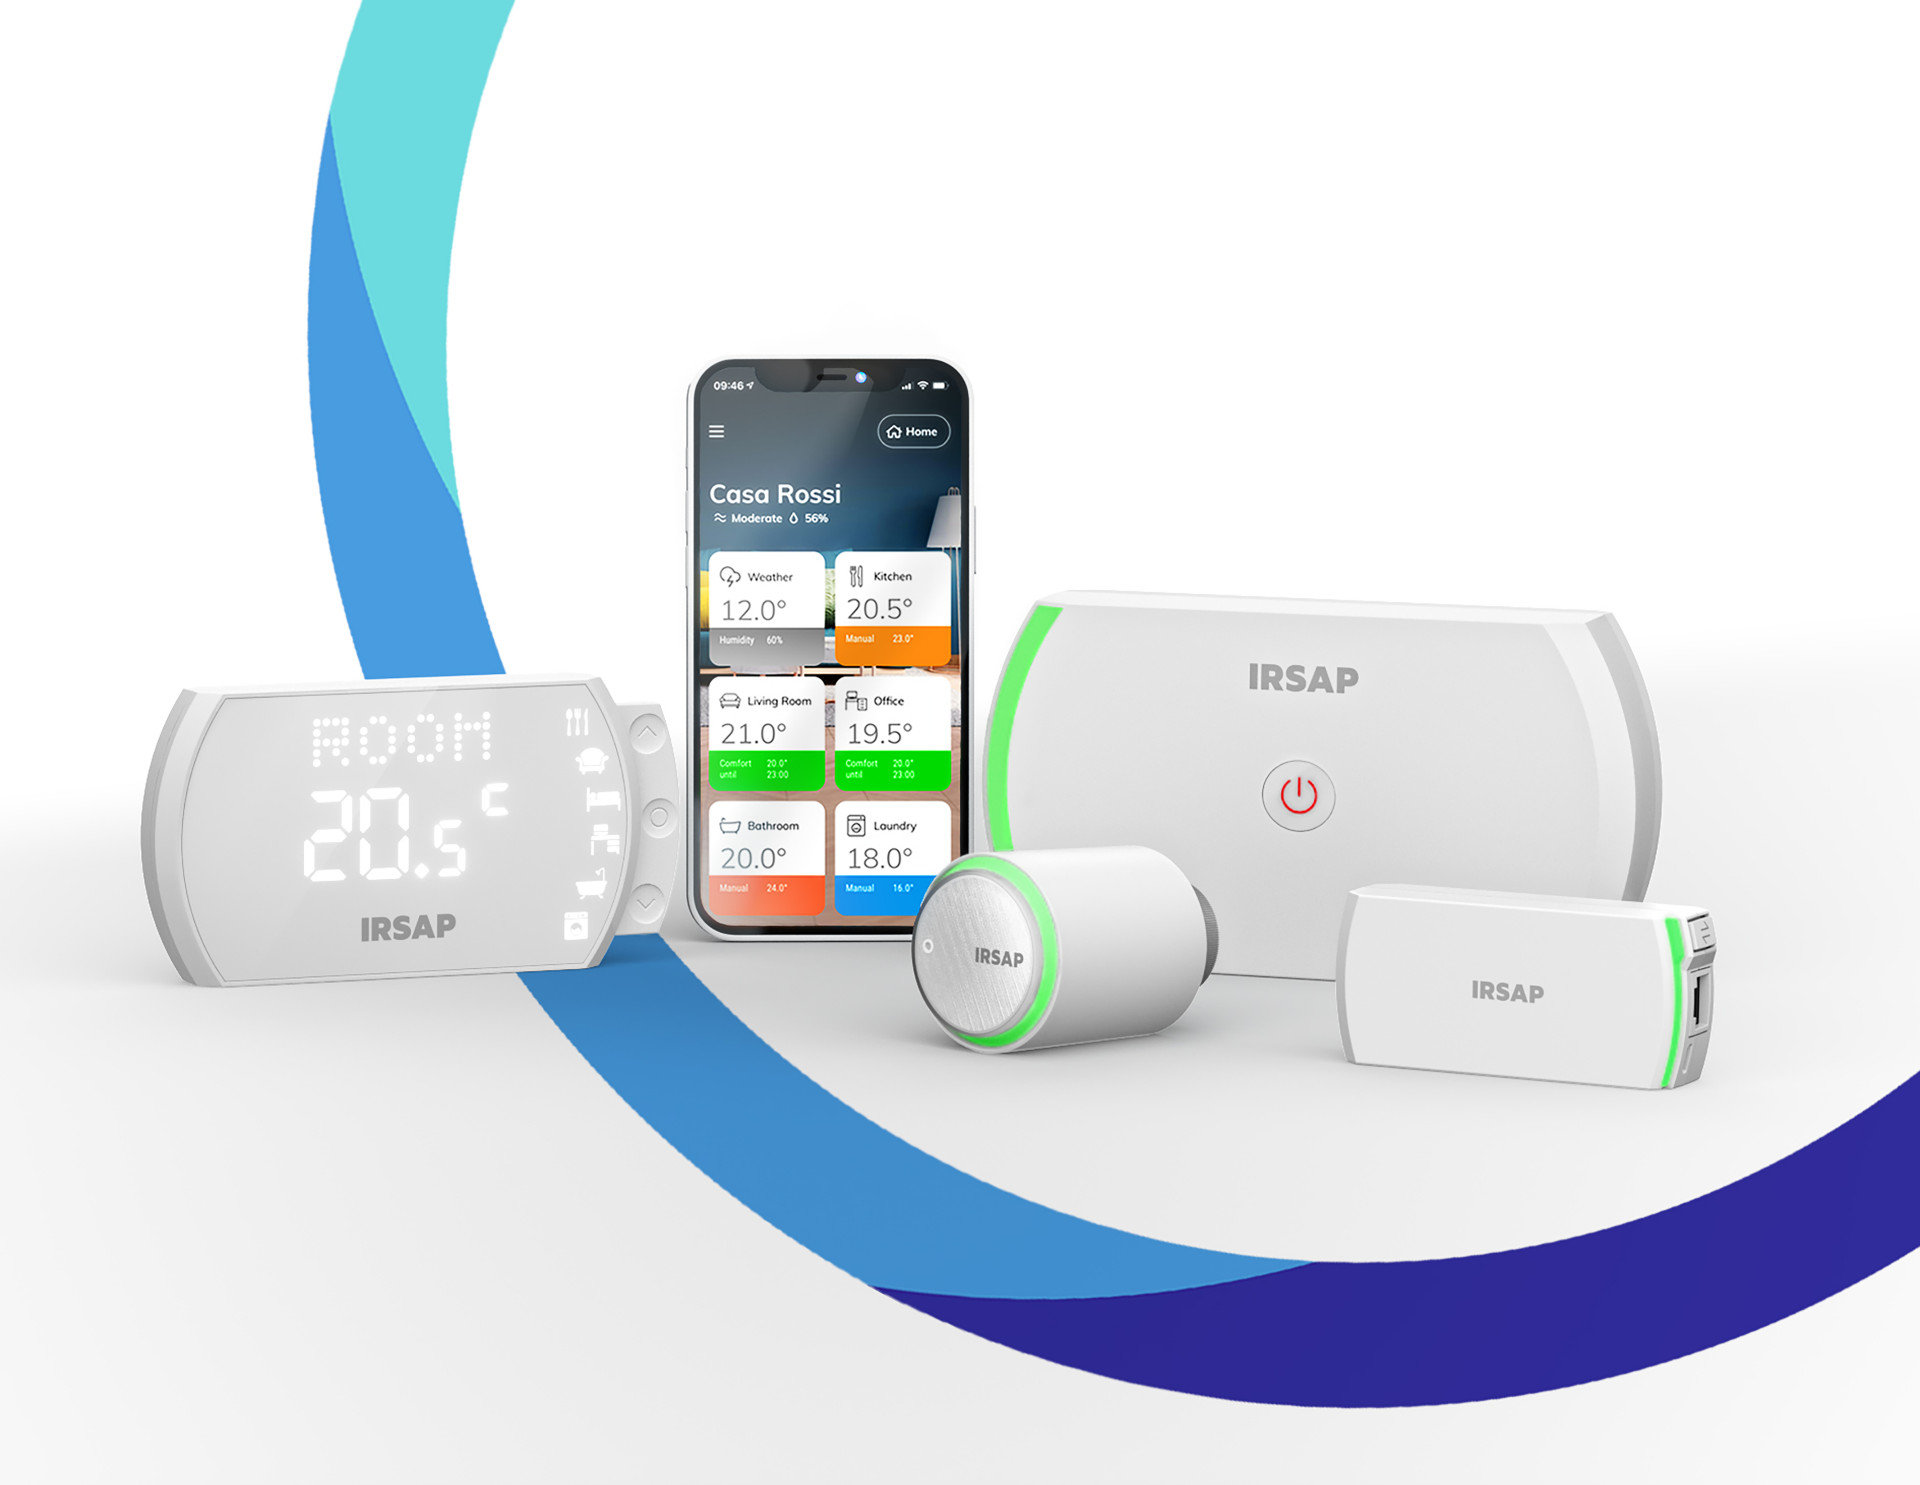
\includegraphics[width=11cm]{img/now.jpeg}
    \caption{Sistema IRSAP NOW per impianti idraulici}
    \label{fig:dispositivi_now}
\end{figure}

Una delle difficoltà attuali è l'impossibilità di andare a testare in maniera isolata i
dispositivi RF e l'unità centrale.

Ad esempio per validare una nuova versoine firmware della CU è necessario avere a disposizione tanti dispositivi quanti
ne supporta al massimo il sistema, ovvero 48, un numero che rende molto complessa anche a
livello logistico l'operazione (si pensi ad es. solo al fatto che questi dispositivi funzoinano a
batterie che dovrebbero essere continuamente mantenute cariche).

Si potrebbe quindi, mediante un'interfaccia radio opportunamente tarata sulle frequenze usate
dal sistema, andare a simulare i dispositivi lato software, consentendo con un'unica interfaccia
radio di simulare tutti i 48 dispositivi senza fisicamente averli in ufficio.

Oltre a ciò in questo progetto si può porsi anche ad un livello più basso: l'unità
centrale contiene due microcontrollori (e di conseguenza due firmware) che comunicano fra di
loro mediante un protocollo seriale (su interfaccia UART). Uno integra il ricetrasmettitore
a radiofrequenza ed è deputato a gestire la comunicazione con i dispositivi
finali, l'altro invece implementa tutte le logiche di funzionamento incluso l'interfacciamento
con il cloud, che avviene tramite porta ethernet.

Si potrebbe quindi andare a testare i due firmware in maniera isolata l'uno dall'altro,
andando a simulare sempre tramite software la controparte mancante. Questo evita di dover
testare tutto i sistema, in particolare la parte RF, quando uno solo dei due software viene
aggiornato. Infatti la parte radio viene aggiornata decisamente più di rado rispetto alla
gestione delle logiche di funzionamento, ma è la più dispendiosa in termini di tempo da testare
(anche perché gestendo a livello fisico la comunicazione RF, in linea teorica, ogni volta andrebbero
rieseguiti i test di laboratorio per assicurarsi che i parametri radio restino nei limiti
imposti dalla normativa vigente).

\section{Test di un termostato}

In IOTINGA infine abbiamo altri progetti firmware più complessi su cui questa metodologia
di test potrebbe essere applicata. Uno su tutti il progetto YAT (Yet Another Thermostat),
un cronotermostato Wi-Fi in grado di comunicare con la caldaia su bus OpenTherm, ma
che in futuro verrà prodotto anche in versione Modbus.

La peculiarità di questo progetto è il fatto che è prevista l'interazione fra più
termostati mediante Bluetooth Low Energy (BLE) in modalità Long Range. In questo modo
si può gestire un impianto multizona, in cui vi è un termostato ``master'' (alimentato
tramite tensione di rete) che mantiene la connessione verso il cloud e la comunicazione
con gli altri termostati ``slave'', che possono essere dei dispositivi a batteria
in quanto non necessitano di una costante connessione con la rete.

Altra caratteristica è un'interfaccia utente (HMI)
locale completa, che utilizza un display a matrice in bianco e nero (o in modelli
futuri a colori TFT) e dei pulsanti capacitivi per navigare nei vari menù. Anche
qui la sfida è riuscire a testare anche l'interfaccia utente in maniera più o meno
automatizzata. Si potrebbe ad esempio escludere completamente il display e verificare
tramite interfacciamento SPI che il microcontrollore arrivi a scrivere i dati correttamente
nella memoria video dello schermo.

Come negli scenari visti fin ora anche qui abbiamo una possibilità di gestire configurazioni
differenti, unita al fatto che questo dispositivo verrà venduto anche in modalità ``white label'',
ossia ogni produttore potrà scegliere di andare a personalizzare alcuni aspetti e quindi
avere un firmware differente dagli altri. Consegue quindi che ad una modifica potrebbe
corrispondere un numero elevato di binari differenti da testare, uno per cliente, e
ancora la necessità di effettuare dei test automatizzati per garantire la qualità di
quanto finisce in mano ai clienti.

\section{Ringraziamenti}

Ringrazio IOTINGA s.r.l, ed in particolare Matteo e Simone, per questi 3 anni di
lavoro assieme, dove ho potuto sperimentare e migliorare la mia conoscenza su un
numero di tecnologie ed ambiti che è impossibile elencare in un paragrafo.

Ringrazio IRSAP s.p.a., ed in particolare Marco, Leandro, Daniele, Mario, e tutto il team
di ``IRSAP NOW'' con cui ho potuto lavorare assieme in questi ultimi anni per realizzare
quanto si è visto solo in piccola parte in questo documento.

\end{document}
